%chapter 8
\chapter{Accident Studies}
\section{Introduction}
The problem of accident is a very acute in highway transportation due to complex flow pattern of vehicular traffic, presence of mixed traffic along with pedestrians. Traffic accident leads to loss of life and property. Thus the traffic engineers have to undertake a big responsibility of providing safe traffic movements to the road users and ensure their safety. Road accidents cannot be totally prevented but by suitable traffic engineering and management the accident rate can be reduced to a certain extent. For this reason systematic study of traffic accidents are required to be carried out. Proper investigation of the cause of accident will help to propose preventive measures in terms of design and control.
\section{Objectives of Accident Studies}
Some objectives of accident studies are listed below:
\begin{itemize}
	\item To study the causes of accidents and suggest corrective measures at potential location;
	\item To evaluate existing design;
	\item To compute the financial losses incurred;
	\item To support the proposed design and provide economic justification to the improvement suggested by the traffic engineer;
	\item To carry out before and after studies and to demonstrate the improvement in the problem.
\end{itemize}
%
\section{Causes of Road Accidents}
The various causes of road accidents are:
\begin{enumerate}
	\item \textbf{\textit{Road Users}} - Excessive speed and rash driving, violation of traffic rules, failure to perceive traffic situation or sign or signal in adequate time, carelessness, fatigue, alcohol,sleep etc.
	\item \textbf{\textit{Vehicle}} - Defects such as failure of brakes, steering system, tyre burst,lighting system.
	\item \textbf{\textit{Road Condition}} - Skidding road surface, pot holes, ruts.
	\item \textbf{\textit{Road design}} - Defective geometric design like inadequate sight distance, inadequate width of shoulders, improper curve design, improper traffic control devices and improper lighting.
	\item \textbf{\textit{Environmental factors}} -unfavorable weather conditions like mist, snow, smoke and heavy rainfall which restrict normal visibility and and makes driving unsafe.
	\item \textbf{\textit{Other causes}} -improper location of advertisement boards, gate of level crossing not closed when required etc..
\end{enumerate}
\section{Accident Analysis}
\subsection{Accident Data Collection}
The accident data collection is the first step in the accident study. The data collection of the accidents is primarily done by the police. Motorist accident reports are secondary data which are filed by motorists themselves. The data to be collected should comprise all of these parameters:
\begin{itemize}
	\item \textbf{\textit{General}} - Date, time, person involved in accident, classification of accident like fatal, serious, minor e.t.c.
	\item \textbf{\textit{Location}} - Description and detail of location of accident.
	\item \textbf{\textit{Details of vehicle involved}} - Registration number, description of vehicle, loading detail, vehicular defects e.t.c.
	\item \textbf{\textit{Nature of accident}} - Details of collision, damages, injury and casualty e.t.c.
	\item \textbf{\textit{Road and traffic condition}} - Details of road geometry, surface characteristics,type of traffic, traffic density e.t.c.
	\item \textbf{\textit{Primary causes of accident}} - Details of various possible cases (already mentioned) which are the main causes of accident.
	\item \textbf{\textit{Accident cost}} - Financial losses incurred due to property damage, personal injury and casualty.
\end{itemize}
These data collected need proper storing and retrieving for the following purpose. The purposes are as follows:
\begin{enumerate}
	\item Identification of location of points at which unusually high number of accident occur.
	\item Detailed functional evaluation of critical accident location to identify the causes of accidents.
	\item Development of procedure that allows identification of hazards before large number of accidents occurs.
	\item Development of different statistical measures of various accident related factors to give insight into general trends, common casual factors, driver profiles, e.t.c.
\end{enumerate}
%
\subsection{Accident Investigation}
The accident data collection involves extensive investigation which involves the following procedure:
\begin{enumerate}
	\item \textbf{\textit{Reporting}}: It involves basic data collection in form of two methods:
		\begin{enumerate}
			\item \textbf{\textit{Motorist accident report}} - It is filed by the involved motorist involved in all accidents fatal or injurious.
			\item \textbf{\textit{Police accident report}} - It is filed by the attendant police officer for all accidents at which an officer is present. This generally includes fatal accidents or mostly accidents involving serious injury required emergency or hospital treatment or which have incurred heavy property damage.
		\end{enumerate}
	\item \textbf{\textit{At Scene-Investigation}}: It involves obtaining information at scene such as measurement of skid marks, examination of damage of vehicles, photograph of final position of vehicles, examination of condition and functioning of traffic control devices and other road equipment.
	\item \textbf{\textit{Technical Preparation}}: This data collection step is needed for organization and interpretation of the study made. In this step measurement of grades, sight distance, preparing drawing of after accident situation, determination of critical and design speed for curves is done.
	\item \textbf{\textit{Professional Reconstruction}}: In this step effort is made to determine from whatever data is available how the accident occurs from the available data. This involves accident reconstruction which has been discussed in the upcoming section in detail. It is professionally referred as determining behavioral or mediate causes of accident.
	\item \textbf{\textit{Cause Analysis}}: It is the effort made to determine why the accident occurred from the data available and the analysis of accident reconstruction studies.
\end{enumerate}
\subsection{Accident Data Analysis}
The purpose is to find the possible causes of accident related to driver, vehicle, and roadway. Accident analyses are made to develop information such as:
\begin{enumerate}
	\item \textbf{\textit{Driver and Pedestrian}} - Accident occurrence by age groups and relationships of accidents to physical capacities and to psychological test results.
	\item \textbf{\textit{Vehicle}} - Accident occurrence related to characteristic of vehicle, severity, location and extent of damage related to vehicles.
	\item \textbf{\textit{Roadway conditions}} - Relationships of accident occurrence and severity to characteristics of the roadway and roadway condition and relative values of changes related to roadways.
\end{enumerate}
It is important to compute accident rate which reflect accident involvement by type of highway. These rates provide a means of comparing the relative safety of different highway and street system and traffic controls. Another is accident involvement by the type of drivers and vehicles associated with accidents.
\subsubsection{Accident Rate per Kilometer:}
On this basis the total accident hazard is expressed as the number of accidents of all types per km of each highway and street classification.
\begin{equation}
	R = \frac{A}{L}
\end{equation}
Where, $ R $ = total accident rate per km for one year, $ A $ = total number of accident occurring in one year, $ L $ = length of control section in km.
%
\subsubsection{Accident Involvement Rate:}
It is expressed as numbers of drivers of vehicles with certain characteristics who were involved in accidents per 100 million vehicle-km of travel.
\begin{equation}
	R = \frac{N \times 10^8}{V}
\end{equation}
Where, $ R $ = accident involvement per 100 million vehicle-km of travel, $ N $ = total number of drivers of vehicles involved in accidents during the period of investigation and $ V $ = vehicle-km of travel on road section during the period of investigation.
%
\subsubsection{Death Rate Based on Population:}
The traffic hazard to life in a community is expressed as the number of traffic fatalities per 100,000 populations. This rate reflects the accident exposure for entire area.
\begin{equation}
	R = \frac{B \times 10^5}{P}
\end{equation}
Where, $ R $ = death rate per 100,000 population, $ B $ = total number of traffic death in one year and $ P $ = population of area.
\subsubsection{Death Rate Based on Registration:}
The traffic hazard to life in a community can also be expressed as the number of traffic fatalities per 10,000 vehicles registered. This rate reflects the accident exposure for entire area and is similar to death rate based on population.
\begin{equation}
	R = \frac{B \times 10^4}{M}
\end{equation}
Where, $ R $ = death rate per 10,000 vehicles registered, $ B $ = total number of traffic death in one year and $ M $ = number of motor vehicles registered in the area.
%
\subsubsection{Accident Based on Vehicle-Km of Travel:}
The accident hazard is expressed as the number of accidents per 100 million vehicle km of travel. The true exposure to accident is nearly approximated by the miles of travel of the motor vehicle than the population or registration.
\begin{equation}
	R = \frac{C \times 10^8}{V}
\end{equation}
Where, R = accident rate per 100 million vehicle km of travel, C = number of total accidents in one year and V = vehicle km of travel in one year.\\\\
%
\textbf{\textit{Numerical Example}}: The Motor vehicle consumption in a city is 5.082 million liters, there were 3114 motor vehicle fatalities, 355,799 motor vehicle injuries, 6,721,049 motor vehicle registrations and an estimated population of 18,190,238. Kilometer of travel per liter of fuel is 12.42 km/liter. Calculate registration death rate, population death rate and accident rate per vehicle km.\\
\textit{Solution}:\\\\
Approximate vehicle km of travel = Total consumption o fuel $ \times $ kilometer of travel per liter of fuel\\
$ \therefore $ Approximate vehicle km of travel = $ 5.08 \times 10^9 \times 12.42 $ = $ 63.1 \times 10^9 $ Km\\\\
now,\\
Registration Death Rate (R) = $ \frac{B \times 10^4}{M} $ = $ \frac{3114 \times 10^4}{6.72 \times 10^6} $ = 4.63\\\\
also,\\
Population Death Rate (R) = $ \frac{B \times 10^5}{P} $ = $ \frac{3144 \times 10^5}{18.2 \times 10^6} $ = 17.1\\\\
also, (total no. of accidents = no. of vehicle fatalities)\\
Accident Rate per Vehicle (R) = $ \frac{C \times 10^8}{V} $ = $ \frac{3114 \times 10^8}{63.1 \times 10^9} $ = 4.93
\section{Accident Reconstruction}
Accident reconstruction deals with representing the accidents occurred in schematic diagram to determine the pre-collision speed which helps in regulating or enforcing rules to control or check movement of vehicles on road at high speed. The following data are required to determine the pre-collision speed:
\begin{enumerate}
	\item Mass of the vehicle
	\item Velocities after collision
	\item Path of each vehicle as it approaches collision point
\end{enumerate}
The collision may be of two types collinear impact or angular collision.
\subsection{Collinear Impact}
A collision is said to be a collinear impact/ collision if the colliding bodies are traveling along the same line of action. Collinear impact can be again divided into two types:
\begin{enumerate}
	\item Rear end collision
	\item Head-on collision
\end{enumerate}
Collinear impact can be defined by two theories, they are:
\begin{enumerate}
	\item Poisson Impact Theory
	\item Energy Theory
\end{enumerate}
\subsubsection{Poisson Impact Theory}
\begin{center}
	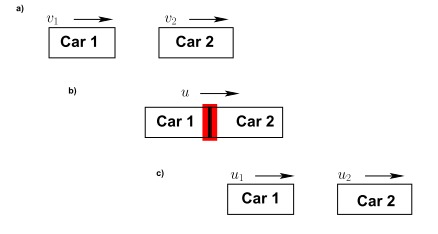
\includegraphics[scale=0.8]{gfx/fig56.png}
\end{center}
Poisson impact theory, divides the impact in two parts - compression and restitution. The Figure above shows two vehicles traveling at an initial speed of $ v_1 $ and $ v_2 $ collide and obtain a uniform speed say u at the compression stage. And after the compression stage is over the final speed is $ u_1 $ and $ u_2 $. The compression phase is cited by the deformation of the cars. From the Newtons law $ F = ma $,
\begin{equation}
	m_1 \frac{dv_1}{dt} \:\: and \:\: m_2 \frac{dv_2}{dt}
\end{equation}
where, $ m_1 $ and $ m_2 $ are the masses of the cars and $ F $ is the contact force. We know that every reaction has equal and opposite action. So as the rear vehicle pushes the vehicle ahead with force $ F $. The vehicle ahead will also push the rear vehicle with same magnitude of force but has different direction. The action force is represented by $ F $, whereas the reaction force is represented by $ -F $ as shown in the figure below. In the compression phase cars are deformed. The compression phase terminates when the cars have equal velocity. Thus the cars obtain equal velocity which generates the following equation:
\begin{center}
	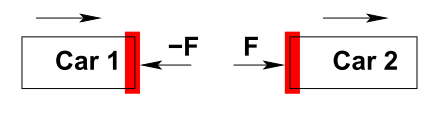
\includegraphics{gfx/fig57.png}
\end{center}
\begin{equation}
	m_1(u - v_1) = -P_c; \:\: m_2(u - v_2) = P_c
\end{equation}
Where, $ P_c \equiv \int_{0}^{\tau_c} F dt $ which is the compression impulse and $ \tau_c $ is the compression time. Thus, the velocity after collision is obtained as:
\begin{equation}
	u = \frac{m_1 v_1 + m_2 v_2}{m_1 + m_2}
\end{equation}
The compression impulse is given by:
\begin{equation}
	P_c = \frac{m_1 m_2}{m_1 + m_2} (v_1 - v_2)
\end{equation}
In the restitution phase the elastic part of internal energy is released,
\begin{gather}
	m_1(u_1 - u) = -P_r\\
	m_2(u_2 - u) = P_r
\end{gather}
Where, $ P_r \equiv \int_{0}^{\tau_r} F dt $ is the restitution impulse and $ \tau_r $ is the restitution time. According to Poisson's hypothesis restitution impulse is proportional to compression impulse.
\begin{equation}
	P_r = e \: P_c
\end{equation}
Restitution impulse $ e $ is given by:
\begin{equation}
	e = \frac{u_2 - u_1}{v_1 - v_2}
\end{equation}
The total impulse is $ P = P_1 + P_2 $,
\begin{equation}
	P = (1 + e) \frac{m_1 m_2}{m_1 + m_2} \Delta v 
\end{equation}
The post impact velocities are given by:
\begin{gather}
	u_1 = u - e \frac{m_2}{m_1 + m_2} \Delta v \: = \: v_1 - (1 + e) \frac{m_2}{m_1 + m_2} \Delta v\\
	u_2 = u + e \frac{m_1}{m_1 + m_2} \Delta v \: = \: v_2 + (1 + e) \frac{m_1}{m_1 + m_2} \Delta v
\end{gather}
Where. $ \Delta v = v_1 - v_2 $. But we are required to determine the pre-collision speed according to which the safety on the road can be designed. So we will determine $ v_1 $ and $ v_2 $ from the given value of $ u_1 $ and $ u_2 $ .\\\\
\textbf{\textit{Numerical Example:}}\\
Two vehicles traveling in the same lane have masses 3000 kg (following) and 2500 kg (leading). Also the velocity of the vehicles after collision is 25 kmph and 56 kmph respectively. The coefficient of restitution of the two vehicle system is assumed to be 0.6. Determine the pre-collision speed of the two vehicles.\\
\textit{Solution}:
mass of the vehicle 1 ($ m_1 $) = 3000 Kg\\
mass of the vehicle 2 ($ m_2 $) = 2500 Kg\\
final speed of the vehicle 1 ($ u_1 $) = 25 kmph\\
final speed of the vehicle 2 ($ u_1 $) = 56 kmph\\
restitution impulse (e) = 0.6\\\\
We have,\\\\
$ 	u_1 = v_1 - (1 + e) \frac{m_2}{m_1 + m_2} (v_1 - v_2) $\\\\
$ 25 = v_1 - (1 + 0.6) \frac{2.5}{3 + 2.5} (v_1 - v_2) $\\\\
$ -1.5 v_1 + 4 v_2 =  137.5 $---------(1)\\\\
Similarly,\\\\
$ 	u_2 = v_2 + (1 + e) \frac{m_1}{m_1 + m_2} (v_1 - v_2) $\\\\
$ 	56 = v_2 + (1 + 0.6) \frac{3}{3 + 2.5} (v_1 - v_2) $\\\\
$ 4.8 v_1 - 0.7 v_2 =  308 $---------(2)\\\\
Solving eqn (1) and (2) we get,\\
$ v_1 $ = 73 kmph, and $ v_2 $ = 62 kmph\\\\
Thus from the result we can infer that the follower vehicle was traveling at quite high speed which may have resulted in the collision. The solution to the problem may be speed restriction in that particular stretch of road where accident occurred.
\subsubsection{Energy Theory}
Applying principle of conservation of energy or conservation of momentum also the initial speed of the vehicle can be computed if the skid marks are known. It is based on the concept that there is reduction in kinetic energy with the work done against the skid resistance. So if the vehicle of weight $ W $ slow down from speed $ v_1 $ to $ v_2 $, then the loss in kinetic energy will be equal to the work done against skid resistance, where work done is weight of the vehicle multiplied by the skid distance and the skid resistance coefficient.
\begin{equation}
	\frac{W \times (v_1^2 - v_2^2)}{2g} = W \times f \times S
\end{equation}
Where, $ f $ is the skid resistance coefficient and $ S $ is the skid distance. It also follows the law of conservation of momentum ($ m_1 $, $ v_1 $ are the mass and velocity of first vehicle colliding with another vehicle of mass and velocity $ m_2 $, $ v_2 $ respectively).
\begin{equation}
	 m_1 v_1 = m_2 v_2
\end{equation}
\textbf{\textit{Numerical Example}}:\\
A vehicle of 2000 kg skids a distance of 36 m before colliding with a stationary vehicle of 1500 kg weight. After collision both vehicle skid a distance of 14 m. Assuming coefficient of friction 0.5, determine the initial speed of the vehicle.\\\\
\textit{Solution}:\\\\
Let the weight of the moving vehicle is $ W_A $, let the weight of the stationary vehicle is $ W_B $, skid distance before and after collision is $ s_1 $ and $ s_2 $ respectively, initial speed is $ v_1 $, speed after applying brakes before collision is $ v_2 $ and the speed of both the vehicles A and B after collision is $ v_3 $, and the final speed $ v_4 $ is 0. Then:\\\\
After Collision:\\\\
Loss in kinetic energy of both cars = Work done against skid resistance\\\\
$ \frac{(W_A + W_B) \times (v_3^2 - v_4^2)}{2g} = (W_A + W_B) \times f \times s_2 $\\\\
$ \frac{v_3^2}{2g} = 0.5 \times 14 $\\\\
$ \therefore v_3 = 11.71 $ m/s \\\\
During Collision:\\\\
Momentum before impact = momentum after impact\\\\
$ \frac{W_A \times v_2}{g} = \frac{(W_A + W_B) \times v_3}{g}$\\\\
$ v_2 = \frac{(2000 + 1500) \times 11.71}{2000} $\\\\
$ \therefore v_2 = 20.5 $ m/s\\\\
Before Collision:\\\\
Loss in kinetic energy of moving vehicle = work done against braking force in reducing the speed\\\\
$ \frac{W_A \times (v_1^2 - v_2^2)}{2g} = W_A \times f \times s_1 $\\\\
$ \frac{(v_1^2 - 20.5^2)}{2 \times 9.81} = 0.5 \times 36 $\\\\
$ \therefore v_1 = 27.8 $ m/s = 100 kmph\\\\
$ \therefore $ The pre-collision speed of the moving vehicle is 100 kmph.
%
\subsection{Angular Collision}

